
Most of the ordinary matter is made up of stable particles. Indeed, rare particles are not easily found since they will decay into ordinary stable matter before they can be observed. The best way to observe unstable or rare particles is at the place and time of their production. Physicists have therefore turned their detectors towards the skies for a time, as the interactions between cosmic rays and the atmosphere can create many of the desired new particles. Even though this approach lead to great discoveries, and to a better understanding of particle physics, ways to produce such processes in a controlled environment can be designed and have many advantages. One of such experiment is the Large Hadron Collider (LHC), which collides protons together with the goal of creating new particles. The LHC apparatus will be presented in section \ref{sec:LHC}. One of the advantages of this experimental context is the possibility of having a global understanding of collision through the detection of most of the outgoing products. The Compact Muon Solenoid (CMS) experiment is a detector placed around of the collision points of the LHC that will provide such detection, and will be presented in section \ref{sec:CMS}. In order to compare and eventually match results with theory, simulation of both the hard processes of the collision and interaction of the products with the detector is then explained in section \ref{sec:cms_physics_event_generation}. Finally, to interpret the signals gathered by the detector, a reconstruction algorithm is applied to both data and simulation, as detailed in section \ref{sec:cms_physics_event_reconstruction}.

\section{The Large Hadron Collider}
\label{sec:LHC}

The LHC is the biggest and most powerful collider in the world. It was built in a 27 km long underground circle cave, over 100m below the surface. It is situated at the Franch-Swiss border on the CERN (European Center of Nuclear Research) campus.

Made of two rings that will each accelerate protons giving them up to 7 TeV of usable energy in the collision, totaling 14 TeV in the centre of mass \cite{Brüning:782076,Brüning:815187,Benedikt:823808}. This acceleration is done through the use of 16 radio frequency cavities, and kept along a circular trajectory by about 9500 magnets. Those magnets are cooled down to 1.8 K thanks to superfluid helium, and through supraconductivity are able to deliver a nominal magnetic field of 8.33 T.

\subsection{Proton acceleration}

Before they reach nominal energy in the LHC rings, protons are gradually accelerated by smaller accelerators :

\paragraph{LINAC 2} is the start of the whole acceleration process. Hydrogen is ionized by an electric field to provide protons accelerated to an energy of 50 MeV.

\paragraph{The Proton Synchrotron Booster (PSB)} is a circular accelerator where the beams of protons reach an energy of 1.4 GeV.

\paragraph{The Proton Synchrotron (PS)} is another circular accelerator, accelerating protons to an energy of 25 GeV.

\paragraph{The Super Proton Synchrotron (SPS)} is the last accelerator before the LHC. Protons will be accelerated to 450 GeV before being injected in the LHC to reach 7 TeV.

A descriptive diagram of the acceleration chain is presented in figure \ref{fig:LHC_acceleration}

\begin{figure}
    \centering
    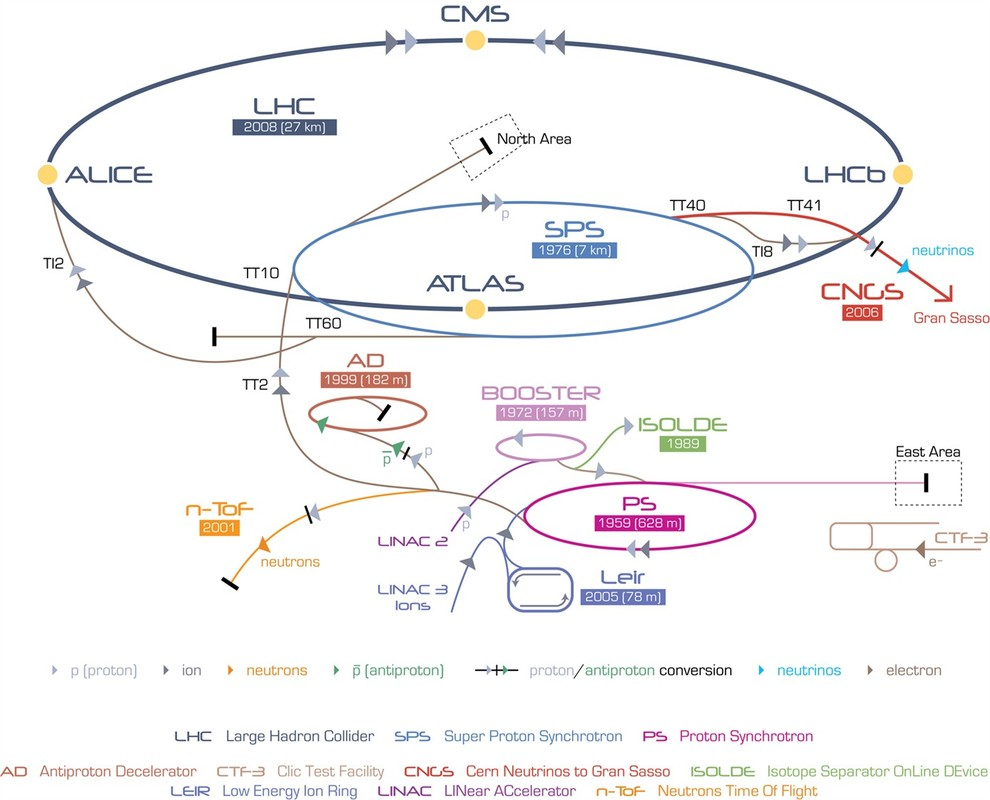
\includegraphics[width=\textwidth]{Images/CERN_accelerators.jpg}
    \caption{Diagrams of the full accelerator complex at CERN, including the LINAC2, BOOSTER (PSB), PS, SPS and LHC accelerators.}
    \label{fig:LHC_acceleration}
\end{figure}

\subsection{Luminosity}

Instantaneous luminosity is a key variable in a collider experiment. Expressed in $\mathrm{cm^{-2} s^{-1}}$, it is proportional to the number of collisions per seconde and per square centimeter. It can be expressed as

\begin{equation}
    \Lagr_{\rm{inst}} = \frac{\gamma f n_p N_p^2}{4\pi \epsilon_n \beta^{*}} = \frac{f n_p N_p^2}{4\pi \sigma_x \sigma_y}
\end{equation}
where $\gamma$ is the Lorentz boost, $f$ is the revolution frequency of the bunches, $n_p$ is the number of bunches, $N_p$ is the number of proton per bunch, $\epsilon_n$ is the transverse emittance which is a measure of the parallelism of the beam, $\beta^*$ is the amplitude function which measures the distance between the interaction point and the place where the beam gets twice as wide, and $\sigma_{x,y}$ the width of each beam at the interaction point.

The integrated luminosity over a period of data-taking is defined by $\Lagr = \int \Lagr_{\rm{inst}} dt$. This variables denotes of the quantity of data, and therefore its statistical potency for the experiments. Indeed, the number of events produced by collisions for a given process is 
\begin{equation}
    N = \Lagr \sigma \mend
\end{equation}
In this equation, $\sigma$ is the cross-section of the considered process. This equation shows that to study rare particles or rare decays, it is beneficial to combine both an important instantaneous luminosity and a long data-taking period.

\subsection{Pile-up}

When bunches of protons meet, several pp interactions can happen. The main interaction is called hard process, and ideally should be the only source of the particles that will be detected. Other collisions, whether elastic or inelastic, introduce extra noise, and can be difficult to separate from the hard process elements. This effect is called pile-up (PU). The number of PU events per collision depends on the LHC configuration. Two types of PU can be distinguish, the in-time PU from other collisions occuring at the same time as the hard process and the out-of-time PU, which originates from leftover activity in the detectors from previously occurring collisions.

\subsection{The experiments}

The LHC is circular, thus allowing easily for several interaction points to be set up along the tunnel. Indeed, 4 major experiments have been set up along the LHC, namely ALICE, ATLAS, CMS and LHCb.

\paragraph{A Large Ion Collider Experiment (ALICE)} This experiment is mainly aimed towards the study of nuclear matter deconfinement, creating quark and gluon plasma. Its data gathering is focused around heavy ion collisions (Pb-Pb or p-Pb), but still uses pp collisions to calibrate the detector.

\paragraph{Large Hadron Collider Beauty} This major experiment of the LHC is dedicated to SM studies as well as CP (charge-parity symmetry) violations studies. This is done through the extensive study of the b quark.

\paragraph{A Toroidal Lhc ApparatuS (ATLAS) / Compact Muon Solenoid (CMS)} Those are the generalist experiments of the LHC. Indeed, ATLAS and CMS physics aim range from the Higgs boson giscovery, which was successfully achieved in 2012, to precision measures of the standard model parameters, while also allowing BSM searches, like dark matter candidates, or extra higgs bosons. The search for a heavy neutral Higgs boson at the CMS experiment is presented in section \ref{sec:Analysis}, while the CMS experiment is detailed in the following section \ref{sec:CMS}.


\section{The Compact Muon Solenoid experiment}
\label{sec:CMS}

\begin{figure}
    \centering
    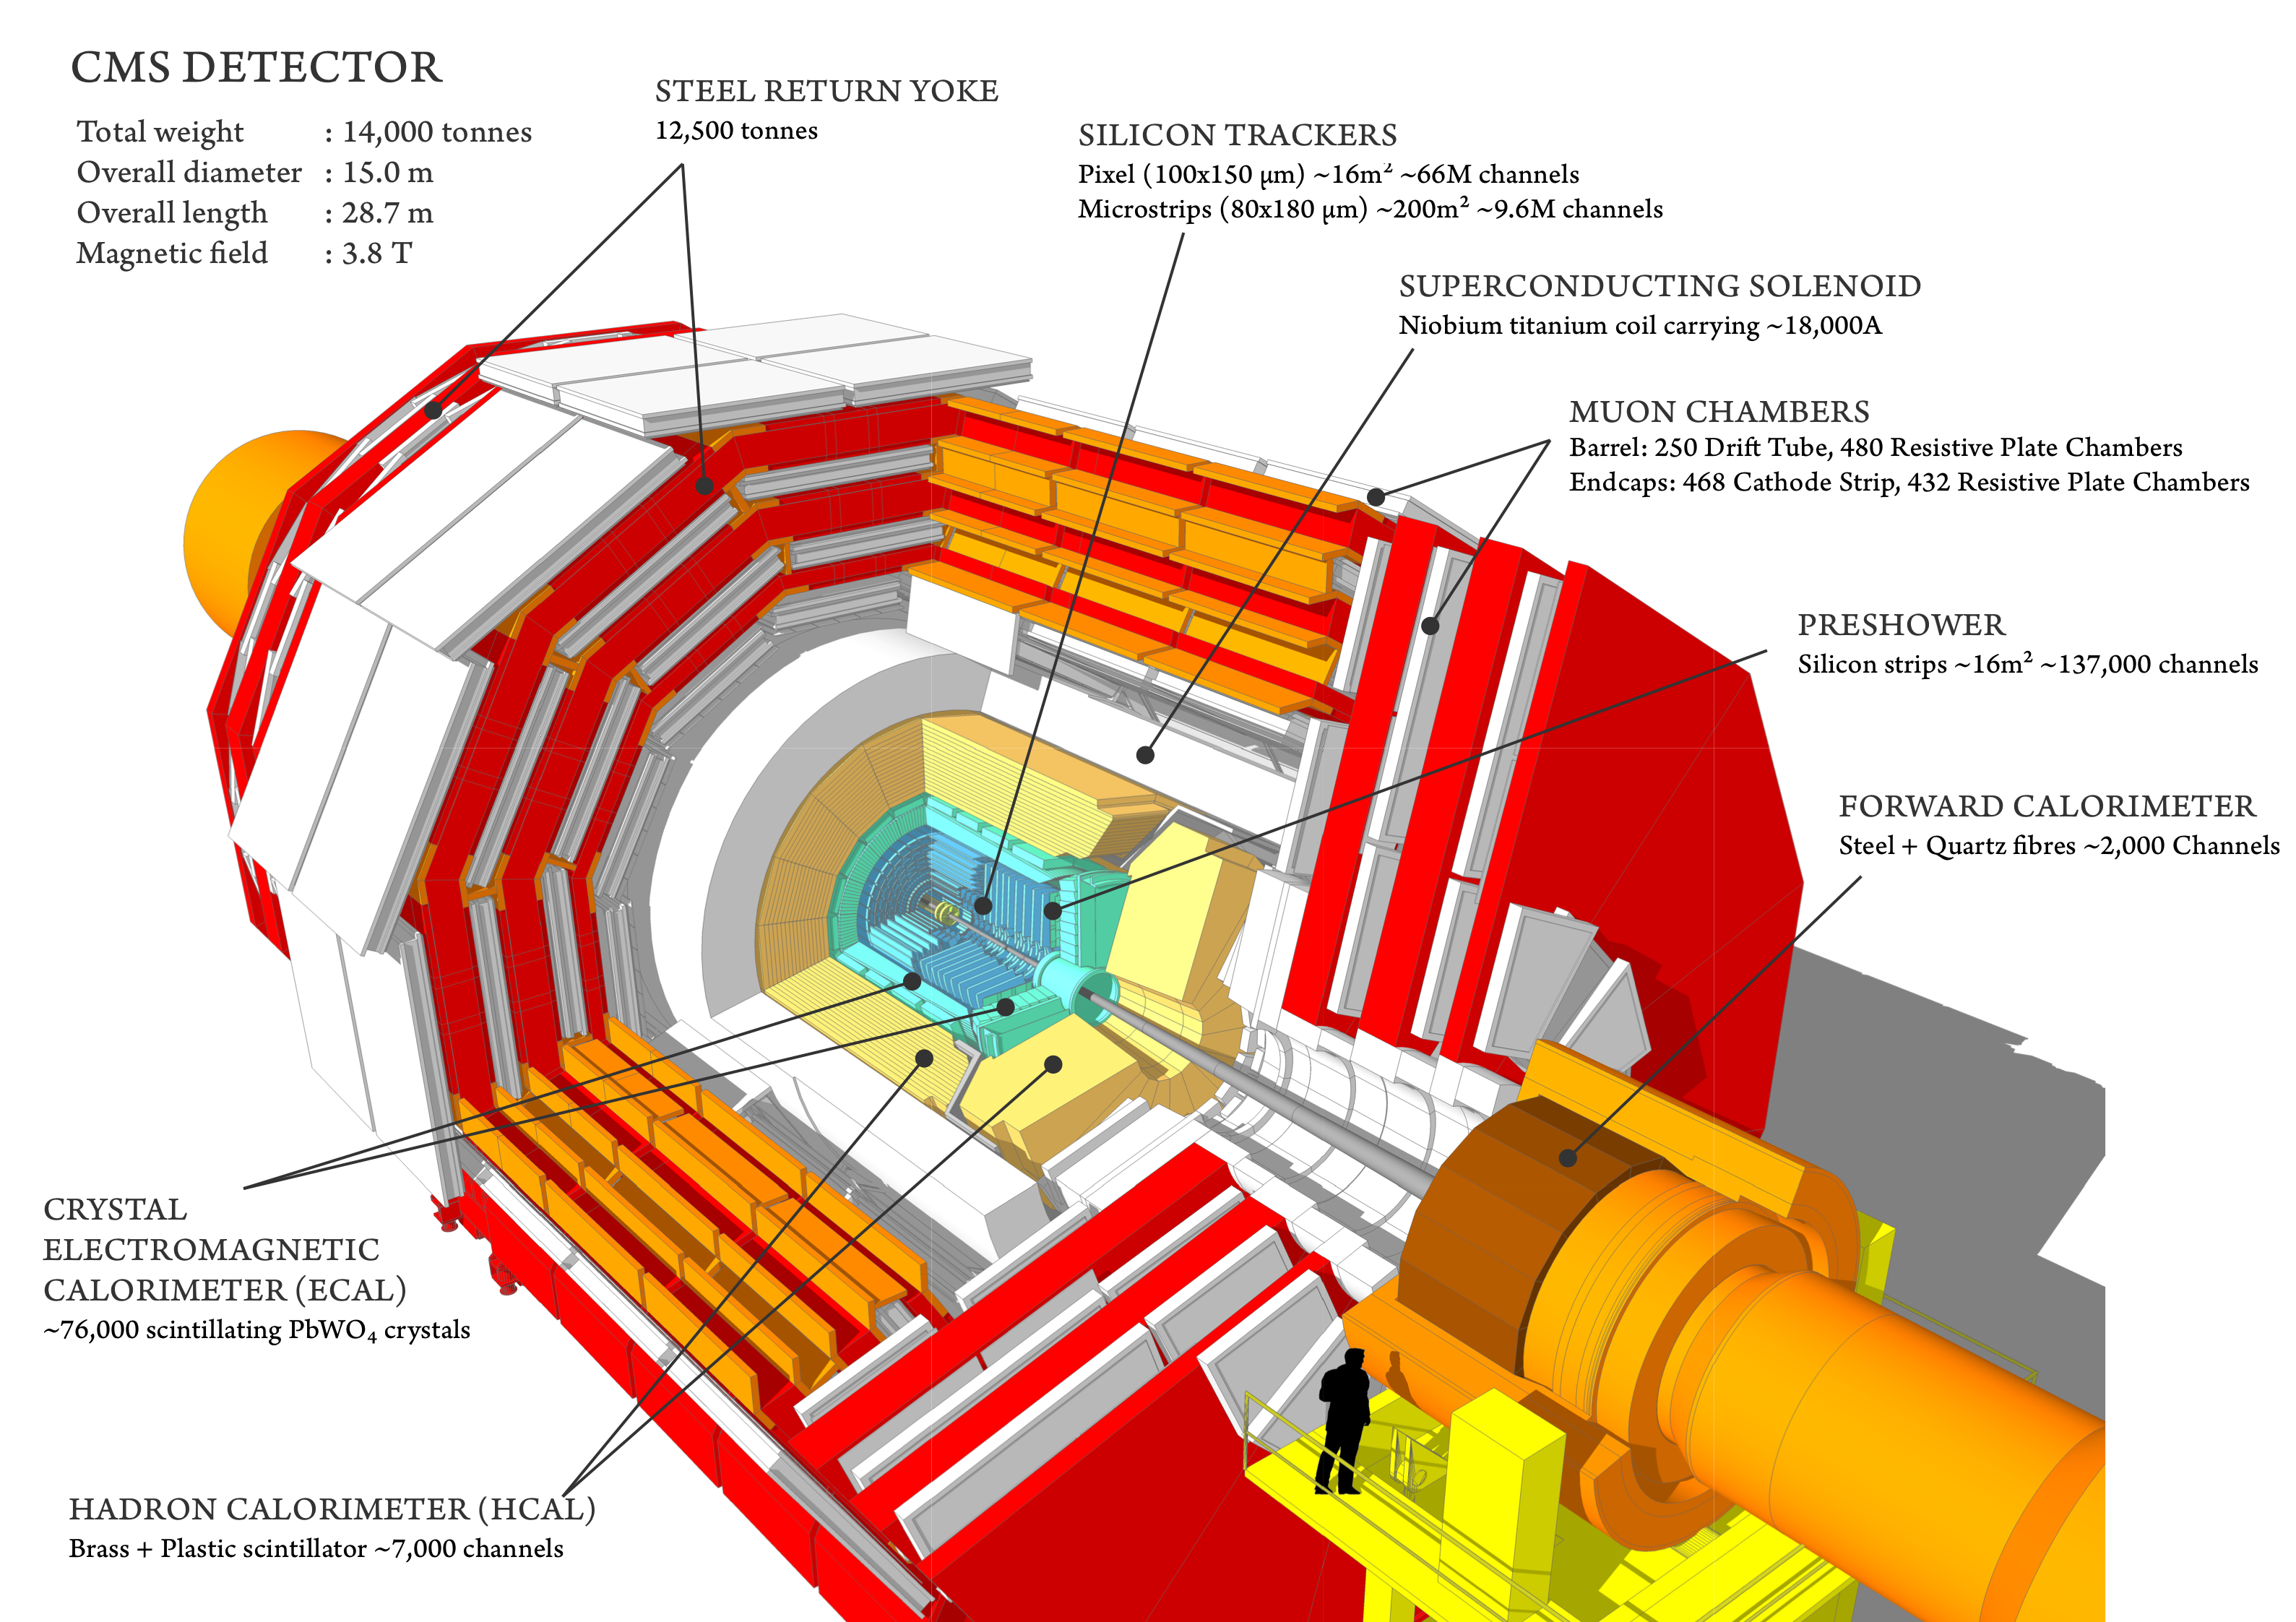
\includegraphics[width=\textwidth]{Images/CMS_subdetectors.png}
    \caption{Illustration of the opened CMS detector and its concentric layers of subdetectors along with the superconducting solenoid and the steel return yoke.}
    \label{fig:CMS_subdetectors}
\end{figure}

The CMS detector is situated in a cavern at LHC point 5, near Meyrin in France. It is a roughly cylindrical-shaped detector of 28.7 m of length and 15 m of diameter, for a weight of 14,000 tons. It is composed of concentric layers, with each layer a different subdetector, with a different role, as illustrated in figure \ref{fig:CMS_subdetectors}. The geometry of the overall detector and of the collisions has pushed to define measurements in terms of a cylindrical frame of reference. First, the z-axis is defined as the beam axis, the x-axis is defined as pointing toward the center of the LHC, and the y-axis as perpendicular to the x and z axis, pointing effectively upward. Then the $\phi$ angle is defined in the (x,y) plane from the x-axis and ranging from $-\pi$ to $\pi$. The $\theta$ angle is defined from the z-axis in the (y,z) plane. But the $\theta$ angle is rarely used and usually replaced by pseudo-rapidity $\eta$, since particle production is constant along $\eta$ and the detection symmetries are then more obvious. $\eta$ can be expressed from $\theta$ as

\begin{equation}
    \eta = - \mathrm{ln} \big[ \mathrm{tan} \big(\frac{\theta}{2}\big)\big] \mend
\end{equation}

Since the LHC is colliding effectively partons within the incoming protons, it is impossible to know the momentum or energy that is available in the collision. But from the LHC geometry, momentum in the transverse plane is by definition null, and from momentum conservation the total momentum of outgoing particles in the transverse plane should be null too. It is then convenient to define the projected energy and momentum in the transverse plane as

\begin{equation}
    p_{\mathrm{T}} = \sqrt{p_{x}^2 p_{y}^2} = \frac{|\Vec{p}|}{\mathrm{cosh} \eta}
\end{equation}
and 
\begin{equation}
    E_{\mathrm{T}} = E \mathrm{sin} \theta = \frac{E}{\mathrm{cosh} \eta} \mend
\end{equation}

One of the objectives of CMS is to measure with great precision the momentum and energies of outgoing particles, even the most boosted ones. To do so, a 3.8 T magnetic field is created thanks to a solenoid. This magnetic field is oriented along the z-axis, to curve the trajectories of charged particles in the transverse plane. In addition to this solenoid, CMS is made up of several subdetectors which goal is to be able to identify, and measure the characteristics, such as the momentum and energies, of all particles flying through. Each layer of detection will be detailed in the following sections, while the reconstruction and identification processes will be detailed in section \ref{sec:cms_physics_event_reconstruction}.

\subsection{The silicon inner tracker}

The full-silicon inner tracking system \cite{Karimäki:368412,CERN-LHCC-2000-016} is the closest layer to the interaction point. It is a cylinder-shaped subdetector with an outer radius of 1.20 m and a length of 5.6 m. The barrel (each of the two endcaps) comprises three (two) layers of pixel detectors, surrounded by ten (twelve) layers of micro-strip detectors. The 16,588 silicon sensor modules are finely segmented into 66 million 150 $\times$ 100 $\mu$m pixels and 9.6 million 80-to-180 $\mu$m-wide strips. Its role is to detect charged particles passing through its different layers in order to reconstruct trajectories. As displayed in figure \ref{fig:tracker_material}, these layers and the pertaining services (cables, support, colling) represent a substantial amount of material in front of the calorimeters, up to 0.5 interaction lengths or 1.8 radiation lengths. The large number of emerging secondary particles turns out to be a major source of complication for reconstruction, but can be mitigated through the use of the combination of information with other subdetectors.

The tracker measures the \pt of charged hadrons at normal incidence with a resolution of 1 $\%$ for $\pt < 20 \mathrm{GeV}$. The relative resolution then degrades with increasing \pt to reach the calorimeter energy resolution for track momenta of several hundred GeV.

\begin{figure}
    \centering
    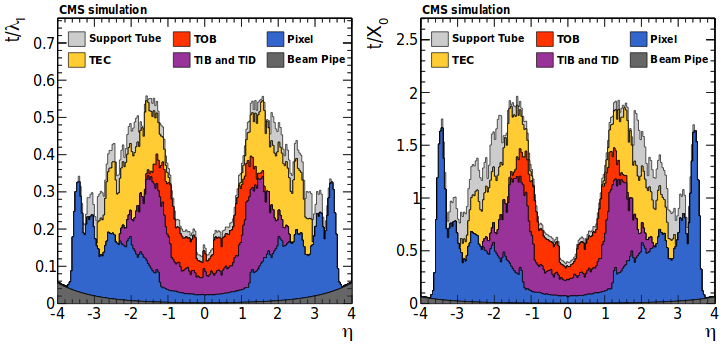
\includegraphics[width=\textwidth]{Images/trackerthickness.png}
    \caption{Total thickness of $t$ of the inner tracker material expressed in units of interaction lengths $\lambda_{l}$ (left) and radiation lengths $X_{0}$ (right), as a function of the pseudorapidity $\eta$. The acronyms TIB, TID, TOB and TEC stand for "tracker inner barrel", "tracker inner disks", "tracker outer barrel", and "tracker endcaps" respectively. The two figures are taken from \cite{Collaboration_2014}.}
    \label{fig:tracker_material}
\end{figure}

\subsection{The electromagnetic calorimeter}

The electromagnetic calorimeter (ECAL) \cite{CERN-LHCC-97-033,Bloch:581342} is a hermetic homogeneous calorimeter made of lead tungstate (PbWO$_4$) crystals. Its role is to stop and measure the energy of electromagnetic particles such as electrons and photons. The barrels covers $|\eta| < 1.479$ and the two endcap disks $1.479 < |\eta| < 3.0$ . The barrel(endcap) crystal length of 23 (22) cm corresponds to 25.8 (24.7) radiation lengths, sufficient to contain more than $98\%$ of the energy of electrons and photons up to 1 TeV. The crystal material also amounts to about one interaction length, causing about two thirds of the hadrons to start showering in the ECAL before entering the next subdetector, the hadronic calorimeter (HCAL).

The crystal transverse size matches the small Molière radius of PbWO$_4$, 2.2 cm. This fine transverse granularity makes it possible to fully resolve hadron and photon energy deposits as close as 5 cm from one another. More specifically, the front face of the barrel crystals has an area of 2.2 $\times$ 2.2 cm$^2$, equivalent to 0.0174 $\times$ 0.0174 in the ($\eta$,$\phi$) plane. In the endcaps, the crystals are arranged instead in a rectangular grid, with a front-face area of 2.9 $\times$ 2.9 cm$^2$. The instrinsic energy resolution of the ECAL barrel was measured with an ECAL supermodule directly exposed to an electron beam, without any attempt to reproduce the material of the tracker in front of the ECAL \cite{Ingram_2007}. The relative energy resolution is parametrized as a function of the electron energy as 

\begin{equation}
    \frac{\sigma}{E} = \frac{2.8\%}{\sqrt{E / \mathrm{GeV}}} + \frac{12\%}{E / \mathrm{GeV}} + 0.3\% \mend
\end{equation}

\subsection{The hadronic calorimeter}

The hadronic calorimeter (HCAL) \cite{CERN-LHCC-97-031} is a hermetic sampling calorimeter consisting of several layers of brass absorber and plastic scintillator tiles. Its role is to stop and measure the energy of outgoing hadrons. It surrounds the ECAL, with a barrel ($|\eta| < 1.3$) and two endcap disks ($1.3 < |\eta| < 3.0$). In the barrel, the HCAL absorber thickness amounts to almost six interaction lengths at normal incidence, and increase to over ten interaction lengths at larger pseudorapidities. It is complemented by a tail catcher (HO), installed outside the solenoid coil. The HO material (1.4 interaction lengths at normal incidence) is used as an additional absorber. At small pseudorapidities ($|\eta| < 0.25$), this thickness is enhanced to a total of three interaction lengths by a 20 cm-thick layer of steel. The total depth of the calorimeter system (including ECAL) is thus extended to a minimum of twelve interaction lengths in the barrel. In the endcaps, the thickness amounts to about ten interaction lengths.

The HCAL is read out in individual towers with a cross section $\delta\eta \times \delta\phi = 0.087 \times 0.087$ for $\eta < 1.6$ and 0.17 $\times$ 0.17 at larger pseudorapidities. The combined (ECAL+HCAL) calorimeter energy resolution was measured in a pion test beam to be 

\begin{equation}
    \frac{\sigma}{E} = \frac{110 \%}{\sqrt{E}} + 9\% \msep
\end{equation}
where $E$ is expressed in GeV.
\subsection{The muon detectors}

Outside the solenoid coil, the magnetic flux is returned through a yoke consisting of three layers of steel interleaved with four muon detector planes \cite{CERN-LHCC-97-032,collaboration_2013}. Drift tude (DT) chamberes and cathode strip chambers (CSC) detect muons in the regions $|\eta| < 1.2$ and $0.9 < |\eta| < 2.4$, respectively, and are complemented by a system of resistive plate chambers (RPC) covering the range $|\eta| < 1.6$. The goal of this subdetector is to detect muons passing through, as muons are the only isolated charged particles expected to go through all the previous layers. Indeed, the reconstruction of muon trajectories, described in section \ref{sec:cms_physics_event_reconstruction}, involves a global trajectory fit across the muon detectors and the inner tracker.

\subsection{The trigger system}
\label{sec:trigger}

At nominal usage, the time between each collision is 25 ns, meaning a frequency of 40 MHz. With an estimated 1 Mo per event, this would lead to a bandwidth of 40 To per second, which is far too much to be handled in real time. In order to limit the bandwidth, a trigger system has been set up, getting rid of fairly common events, which have been already well studied, and storing only events with characteristics that are considered to be relevant. This trigger system has two distinct levels called the level-1 (L1) and high-level (HLT)

\paragraph{Level-1 trigger (L1} This trigger level has the goal of reducing the 40MHz bandwidth into a 100 kHz bandwidth. It does so by relying on ultra-fast electronic hardware, using inputs straight from the muon chambers and calorimeters. The decision to keep or reject an event is then taken in less than 3.2 $\mu$s. 

\paragraph{High level trigger (HLT)} The goal of this level is to reduce the bandwidth to about 100 Hz in order to be able to store the data. This triggering is done on a computer farm installed in a room adjacent to the detector. This allows for more complex triggering algorithms to be used, and even to perform physics object reconstruction. Several trigger algorithms are implemented, usually based on certain physics object requirements, and can be evaluated simultaneously.

\section{Simulation}

In order to be able to compare experimental results with theoretical predictions, both the collision process and the interaction of the outgoing particles with the subdetectors needs to be simulated. The hard process is simulated with an Monte Carlo event generators, which simulates the partons interaction and gives as output the outgoing particles. Then the flight of each particles trough the different subdetectors is extrapolated, and finally the interactions and subdetector outputs is simulated too.

\subsection{Physics event generation} 
\label{sec:cms_physics_event_generation}

As seen before, when two protons collide, only the constituents, namely the partons, will actually collide. Each parton carries a fraction $x$ of the total momentum of the incoming protons. The hard process is described analytically using pertubative theory. A generator will then determine the transition matrix between initial anf final state, following the feynman rules. The leading order calculation is available for most processes, the the following orders are only available for specific subset of processes. Leading order processes are computed using software like MadGraph \cite{Alwall2011}, while next-to-leading order computations are done using software like Powheg \cite{Alioli2010} or MC@NLO \cite{Frixione_2002}.
Those generators will then provide as output the quadri-moment of the outgoing particles produced at the collision.

Particles holding a colour charge that are produced in the collision will radiate gluons and photons. Those gluons can themselves radiate other gluons, creating a cascade. Once the gcreated gluons reach a threshold dictated by the generator, gluons then decay. Since they are subjected to the strong interaction, coloured particles that are created will hadronise, leading to colour-neutral hadrons. This hadronisation happens roughly $5 \times 10^{-24}$ after the coloured particles are produced. But there is no theory describing hadronisation, only phenomenological models. Those models can be separated into two distinct classes: Lund string models \cite{1983PhR....97...31A} and cluster hadronisation based models \cite{Winter2004}. The first uses colour links between partons: when a parton pair get far from each other, the amount of energy rises, until being high enough to create a quark-antiquark pair. This breaks the link and creates two new ones, linking the old particles to the new ones. The cluster hadronisation models use quantum numbers conservation between partons and hadrons.  Parton clusters are created, neutral from a QCD point of vue. A cluster is identified as a hadron if its mass is close to a known hadron. If not, it is considered as a resonance of two lighter hadrons. The created particles can be stable or not. In case of instability, those hadrons decay following the experimentally measured branching ratios.

Those effects are hard to simulate, since the energy scale at which they happen makes QCD non-perturbative. Nevertheless, dedicated software allow to simulate the whole hadronisation chain, each using specific algorithms to simulate this hadronisation chain, for example Pythia \cite{SJOSTRAND2008852} and Herwig \cite{Bellm2016}.

\subsection{Subdetectors and interactions}

Once the outgoing particles have been obtained, the response of the different subdetectors to the particles stable enough to reach them must be simulated. This level of simulation includes the flight of the particles through the subdetectors, the electromagnetic and hadronic cascades, the interaction between particles and the matter of the subdetectors, the electrical response of the subdetectors, and the decay of the particles whose mean life time leads them to decay within the detector geometry. Two approaches are available, a detailed simulation based on Geant4 \cite{AGOSTINELLI2003250}, which is very computationally heavy, and a light simulation, allowing for less precise but faster simulation.

The first simulation relies on a very detailed description of the subdetectors. Indeed, even the cables and hardware material are included in this 3D simulation. This is then used by the Geant4 software, which will simulate the propagations, interactions, scatterings and detection of each subdetectors.

In order to avoid a computational costs and time, a fast simulation has also been made for CMS \cite{Abdullin_2011}. This simulation relies on a simplified geometry of the subdetectors, and considers the material of the subdetectors from a parametrised mean density. The precision level of this simulation is of the percent level, while greatly reducing computational time and efforts. It is therefore very useful in the case of detector modification studies.

\section{Event reconstruction}
\label{sec:cms_physics_event_reconstruction}

\begin{figure}
    \centering
    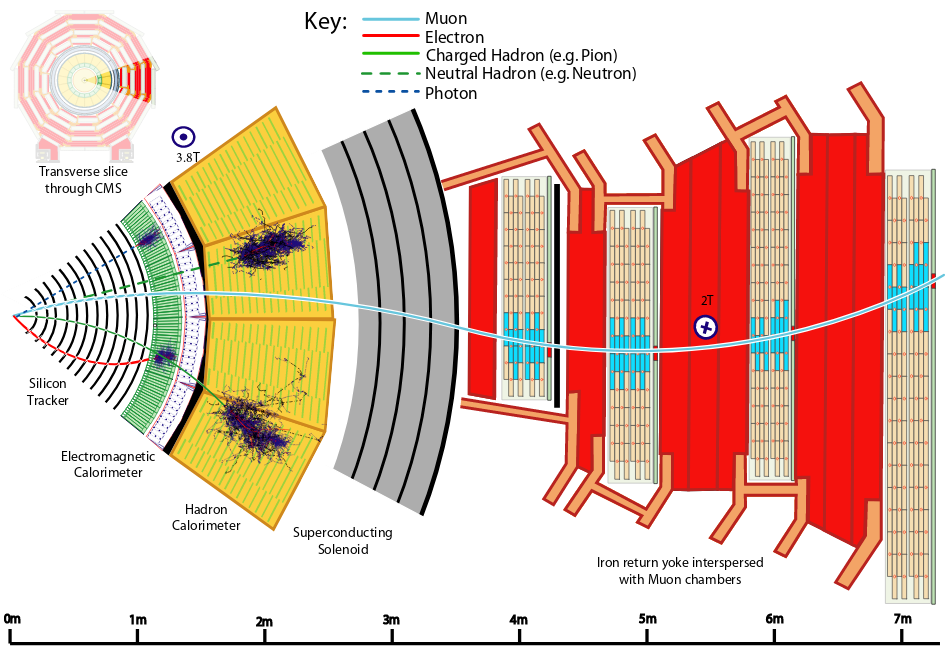
\includegraphics[width=\textwidth]{Images/pflow_illustration_2.png}
    \caption{A sketch of the specific particle interactions in a transverse slice of the CMS detector,from the beam interaction region to the muon detector.  The muon and the charged pion are positively charged, and the electron is negatively charged.}
    \label{fig:pflow_illustration}
\end{figure}

At this point, the signals delivered by the different subdetectors, whether in simulation or data, is hard to interpret. In order to make sense on a physics level of the detection, event reconstruction is developed, its goal is to provide the list of outgoing particles from the collision from the detection data. Event reconstruction is done identically for both simulated events and actual data. In the CMS experiment, this reconstruction is done by a algorithm specifically developed to maximize the usage of the combined information gathered by all subdetectors, as some particles can interact with several subdetector, as illustrated in figure \ref{fig:pflow_illustration}. This algorithm is called the particle-flow algorithm (PF). 

\label{sec:pf}

The PF algorithm can be split into two disctinct steps: first the reconstruction of the elements that will then be used to identify and reconstruct particles.

\subsection{PF elements}

\subsubsection{Charged-particle tracks and vertices}
An iterative process is first used to reconstruct tracks \cite{Collaboration_2014}. This is done using a combinatorial track finder based on Kalman Filtering (KF) with the goal of having as high as possible purity while keeping a moderate efficiency. At each step, the reduction of the misreconstruction is accomplished with quality criteria on the track seeds, on the track vertices, and on the track compatibility with the reconstructed primary vertices, adapted to the track $p_{\mathrm{T}}$, $|\eta|$ and number of hits $n_{\mathrm{hits}}$. The hits associated with the selected tracks are masked in order to reduce the probability of random hit-to-seed association in the next iteration. The remaining hits may thus be used in the next iteration to form new seeds and tracks with relaxed quality criteria, increasing in turn the total tracking efficiency without degrading the purity. The same operation is repeated several times with progressively more complex and time-consuming seeding, filtering, and tracking algorithms.

Nuclear interactions in the tracker material may lead to either a kink in the original hadron trajectory, or to the production of a number of secondary particles. A dedicated algorithm was thus developed to identify tracks linked to a common secondary displaced vertex within the tracker volume \cite{CMS-PAS-TRK-10-003,Khachatryan2010}.

\subsubsection{Tracking for electrons}

Electron reconstruction, originally aimed at characterizing energetic, well-isolated electrons, is naturally based on the ECAL measurements. More specifically, the traditional electron seeding strategy (hereafter called the ECAL-based approach) \cite{2015} makes use of energetic ECAL clusters ($E_{\mathrm{T}}>4 \mathrm{GeV}$).  The cluster energy and position are used to infer the position of the hits expected in the innermost tracker layers under the assumptions that the cluster is produced either by an electron or by a positron.  Because of the significant tracker thickness, most of the electrons emit a sizeable fraction of their energy in the form of bremsstrahlung photons before reaching the ECAL. The performance of the method therefore depends on the ability to gather all the radiated energy, and only that energy.  The energy of the electron and of possible bremsstrahlung photons is collected by grouping into a supercluster the ECAL clusters reconstructed in a small window in $\eta$ and an extended window in $\phi$ around the electron direction (to account for the azimuthal bending of the electron in the magnetic field).

The iterative tracking is designed to have a large efficiency for electrons that can be easily missed by the ECAL-based approach. All the tracks from the iterative tracking are therefore used as potential seeds for electrons, if their $p_{\mathrm{T}}$ exceeds 2 GeV. The large probability for electrons to radiate in the tracker material is exploited to disentangle electrons from charged hadrons. When the energy radiated by the electron is small, the corresponding track can be reconstructed across the whole tracker with a well-behaved $\chi^2$ and be safely propagated to the ECAL inner surface, where it can be matched with the closest ECAL cluster as will be detailed later.  For these tracks to form an electron seed, the ratio of the cluster energy to the track momentum is required to be compatible with unity. In the case of soft photon emission, the pattern recognition may still succeed in collecting most hits along the electron trajectory, but the track fit generally leads to a large $\chi^2$ value.  When energetic photons are radiated, the pattern recognition may be unable to accommodate the change in electron momentum, causing the track to be reconstructed with a small number of hits. A preselection based on the number of hits and the fit $\chi^2$ is therefore applied and the selected tracks are fit again with a Gaussian-sum filter (GSF) \cite{Adam_2005}. The GSF fitting is more adapted to electrons than the KF used in the iterative tracking, as it allows for sudden and substantial energy losses along the trajectory. A final requirement is applied to the score of a boosted-decision-tree (BDT) classifier that combines the discriminating power of the number of hits, the $\chi^2$ of the GSF track fit and its ratio to that of the KF track fit, the energy lost along the GSF track, and the distance between the extrapolation of the track to the ECAL inner surface and the closest ECAL cluster. The tracker-based seeding is also effective at selecting electrons and positrons from conversions in the tracker material, for both prompt and bremsstrahlung photons.  The recovery of the converted photons of the latter category and their association to their parent electrons is instrumental in minimizing energy double counting in the course of the PF reconstruction.


\subsubsection{Tracking for muons}

 The  muon  spectrometer  allows muons to be identified with high efficiency over the full detector acceptance.  A high purity is granted by the upstream calorimeters, meant to absorb other particles (except neutrinos).  The inner tracker provides a precise measurement of the momentum of these muons.  The high-level muon physics objects are reconstructed in a multifaceted way, with the final collection being composed of three different muon types:
 
 \begin{itemize}
     \item standalone muon.  Hits within each DT or CSC detector are clustered to form track segments,  used as seeds for the pattern recognition in the muon spectrometer,  to gather all DT, CSC, and RPC hits along the muon trajectory.  The result of the final fitting is called a standalone-muon track.
     \item global muon.  Each standalone-muon track is matched to a track in the inner tracker(hereafter referred to as an inner track) if the parameters of the two tracks propagated onto a common surface are compatible.  The hits from the inner track and from the standalone-muon track are combined and fit to form a global-muon track.
     \item tracker muon. Each inner track with $p_{\mathrm{T}}$ larger than 0.5 GeV and a total momentum pin excess of 2.5 GeV is extrapolated to the muon system. If at least one muon segment matches the extrapolated track, the inner track qualifies as a tracker muon track.
 \end{itemize}
 
 Charged hadrons may be misreconstructed as muons e.g. if some of the hadron shower remnants reach the muon system (punch-through).  Different identification criteria can be applied to the muon tracks in order to obtain the desired balance between identification efficiency and purity. 

\subsubsection{Calorimeter clusters}

The purpose of the clustering algorithm in the calorimeters is fourfold: detect and measure the energy and direction of stable neutral particles such as photons and neutral hadrons; separate these neutral particles from charged hadron energy deposits; reconstruct and identify electrons and all accompanying bremsstrahlung photons; and help the energy measurement of charged hadrons for which the track parameters were not determined accurately, which is the case for low-quality and high-$p_{\mathrm{T}}$ tracks. The clustering is performed separately in each detector: ECAL barrel and endcaps, HCAL barrel and endcaps, ... The values of all parameters of the clustering algorithm result from optimizations based on the simulation of single photons, \pizero, $K^0_{\mathrm{L}}$ and jets.

First,cluster seeds are identified as cells with an energy larger than a given seed threshold, and larger than the energy of the neighbouring cells. The cells considered as neighbours are either the  four  closest  cells,  which  share  a  side  with  the  seed  candidate,  or  the  eight  closest  cells,including cells that only share a corner with the seed candidate. Second,topological clusters are grown from the seeds by aggregating cells with at least a corner in common with a cell already in the cluster and with an energy in excess of a cell threshold set to twice the noise level. In the ECAL endcaps, because the noise level increases as a function ofθ, seeds are additionally required to satisfy a threshold requirement on $E_{\mathrm{T}}$.

An expectation-maximization algorithm based on a Gaussian-mixture model is then used to reconstruct the clusters within a topological cluster.  The Gaussian-mixture model postulate sthat the energy deposits in the M individual cells of the topological cluster arise from N Gaussian energy deposits where N is the number of seeds.  The parameters of the model are the amplitude $A_i$ and the coordinates in the ($\eta$,$\phi$) plane of the mean $\Vec{\mu}_i$ of each Gaussian, while the width $\sigma$ is fixed to different values depending on the considered calorimeter. The expectation-maximization algorithm is an iterative algorithm with two steps at each iteration.  During the first step, the parameters of the model are kept constant and the expected fraction $f_{ij}$ of the energy $E_j$ measured in the cell at position $\Vec{c_j}$ arising from the $i$th Gaussian energy deposit is calculated as

\begin{equation}
    f_{ij} = \frac{A_i e^{-(\Vec{c_j}-\Vec{\mu}_i)^2 / (2\sigma^2)}}{\sum_{k=1}^N A_k e^{-(\Vec{c_j}-\Vec{\mu}_k)^2 / (2\sigma^2)}} \mend
\end{equation}

The parameters of the model are determined during the second step in an analytical maximum-likelihood fit yielding

\begin{equation}
    A_i = \sum_{j=1}^M f_{ij}E_j , \Vec{\mu}_i = \sum_{j=1}^M f_{ij}E_j \Vec{c_j} \mend
\end{equation}

The energy and position of the seeds are used as initial values for the parameters of the corresponding Gaussian functions and the expectation maximization cycle is repeated until convergence.  To stabilize the algorithm, the seed energy is entirely attributed to the corresponding Gaussian function at each iteration.

\subsubsection{Calorimeter cluster calibration}

In the PF reconstruction algorithm, photons and neutral hadrons are reconstructed from calorimeter clusters. Calorimeter clusters separated from the extrapolated position of any charged-particle track in the calorimeters constitute a clear signature of neutral particles.  On the other hand, neutral-particle energy deposits overlapping with charged-particle clusters can only be detected  as  calorimeter  energy  excesses  with  respect  to  the  sum  of  the  associated  charged-particle momenta. An accurate calibration of the calorimeter response to photons and hadrons is instrumental in maximizing the probability to identify these neutral particles while minimizing the rate of misreconstructed energy excesses, and to get the right energy scale for all neutral particles. A first estimate of the absolute calibration of the ECAL response to electrons and photons, as well as of the cell-to-cell relative calibration, has been determined with test beam data, radioactive sources,  and cosmic ray measurements,  all of which were collected prior to the start of collision data taking.  The ECAL calibration was then refined with collision data collected at $\sqrt{s}=$7 and 8 TeV \cite{2013}. Hadrons generally deposit energy in both ECAL and HCAL. The initial calibration of the HCAL was realized with test beam data for 50 GeV charged pions not interacting in the ECAL, but the calorimeter response depends on the fraction of the shower energy deposited in the ECAL, and is not linear with energy. The ECAL and HCAL cluster energies therefore need to be substantially recalibrated to get an estimate of the true hadron energy. The calibrated calorimetric energy associated with a hadron is expressed as
\begin{equation}
    E_{\mathrm{calib}} = a + b(E)f(\eta)E_{\mathrm{ECAL}} + c(E)g(\eta)E_{HCAL} \msep
\end{equation}
where $E_{\mathrm{ECAL}}$ and $E_{\mathrm{HCAL}}$ are the calibrated energies measured in the ECAL and HCAL, and where $E$ and $\eta$ are the true energy and pseudorapidity of the hadron. To avoid the need for an accurate estimate of the true hadron energy $E$ (which might not be available in real data),  the constant $a$ is chosen to minimize the dependence on $E$ of the coefficients $b$ and $c$. Isolated charged hadrons selected from early data recorded at $\srqt{s}=$ 0.9, 2.2, and 7 TeV have been used to check that the calibration coefficients determined from the simulation are adequate for real data.

\subsection{Particle identification and reconstruction}

\subsubsection{Link algorithm}
A given particle is, in general, expected to give rise to several PF elements in the various CMS subdetectors. The reconstruction of a particle therefore first proceeds with a link algorithm that connects the PF elements from different subdetectors. The probability for the algorithm to link elements from one particle only is limited by the granularity of the various subdetectors and by the number of particles to resolve per unit of solid angle. The probability to link all elements of a given particle is mostly limited by the amount of material encountered upstream of the calorimeters and the muon detector, which may lead to trajectory kinks and to the creation of secondary particles. The link algorithm can test any pair of elements in the event. In order to prevent the computing time of the link algorithm from growing quadratically with the number of particles, the pairs of elements considered by the link procedure are restricted to the nearest neighbours in the ($\eta$,$\phi$) plane. If two elements are found to be linked, the algorithm defines a distance between these two elements aimed at quantifying the quality of the link. The link algorithm then produces PF blocks of elements associated either by a direct link or by an indirect link through common elements. Tracks are linked with clusters if their extrapolated trajectory matches the position of considered clusters. In case several HCAL clusters are linked to the same track, or if several tracks are linked to the same ECAL cluster, only the link with the smallest distance is kept. To collect the energy of photons emitted by electron bremsstrahlung, tangents to the GSF tracksare extrapolated to the ECAL from the intersection points between the track and each of the tracker  layers. A cluster is linked to the track as a potential bremsstrahlung photon if the extrapolated tangent position is within the boundaries of the cluster. Calorimeter cluster-to-cluster links are sought between HCAL clusters and ECAL clusters by checking whether one cluster's position is within another's envelope. Charged-particle tracks may also be linked together through a common secondary vertex, for nuclear-interaction reconstruction. The relevant displaced vertices are retained if they feature at least three tracks. All the tracks sharing a selected nuclear-interaction vertex are linked together. Finally, a link between a track in the central tracker and information in the muon detector is established to form global and tracker muons.

\subsubsection{Muons} First, muon identification proceeds by a set of selections based on the global and tracker muon properties. Isolated global muons are first selected by considering additional inner tracks and calorimeter energy deposits close to its trajectory to carry less than 10$\%$ of the muon \pt, which is sufficient to adequately reject hadrons that would be misidentified as muons. For nonisolated global muons, the tight-muon selection \cite{collaboration_2012} is applied. The PF elements that make up these identified muons are masked against further processing in the corresponding PF block, i.e. are not used as building elements for other particles.

\subsubsection{Electrons and isolated photons} Electron reconstruction is based on combined information from the inner tracker and the calorimeters. Due to the large amount of material in the tracker, electrons often emit bremsstrahlung photons and photons often convert to e$^+$e$^-$ pairs, which in turn emit bremsstrahlung photons,etc.  For this reason, the basic properties and the technical issues to be solved for the tracking and the energy deposition patterns of electrons and photons are similar. Isolated photon reconstruction is therefore conducted together with electron reconstruction. In a given PF block, an electron candidate is seeded from a GSF track, provided that the corresponding ECAL cluster is not linked to three or more additional tracks. A photon candidate is seeded from an ECAL supercluster with \et larger than 10 GeV, with no link to a GSFtrack. For ECAL-based electron candidates and for photon candidates, the sum of the energies measured in the HCAL cells with a distance to the supercluster position smaller than 0.15 in the ($\eta$,$\phi$) plane must not exceed 10$\%$ of the supercluster energy. The total energy of the collected ECAL clusters is corrected for the energy missed in the association process, with analytical functions of $E$ and $\eta$. The final energy assignment for electrons is obtained from a combination of the corrected ECAL energy with the momentum of the GSF track and the electron direction is chosen to be that of the GSF track. Electron candidates must satisfy additional identification criteria in the form of a BDT score and associated working points. This BDT takes up to fourteen variables of the electron candidate and is trained separately for ECAL barrel and endcaps, and for isolated and nonisolated electrons. Photon candidates are retained if they are isolated from other tracks and calorimeter clusters in the event, and if the ECAL cell energy distribution and the ratio between the HCAL and ECAL energies are compatible with those expected from a photon shower. 

\subsubsection{Hadrons and nonisolated photons} 
Once muons, electrons, and isolated photons are identified and removed from the PF blocks,the remaining particles to be identified are charged hadrons, neutral hadrons, nonisolated photons, and more rarely additional muons. The ECAL and HCAL clusters not linked to any track give rise to photons and neutral hadrons. Each of the remaining HCAL clusters of the PF block is linked to one or several tracks (not linked to any other HCAL cluster) and these tracks may in turn be linked to some of the remaining ECAL clusters (each linked to only one of the tracks). If the calibrated calorimetric energy is in excess of the sum of the track momenta by an amountlarger than the expected calorimetric energy resolution for hadrons, the excess may be interpreted as the presence of photons and neutral hadrons. If the calibrated calorimetric energy is compatible with the sum of the track momenta, no neutral particle is identified.  The charged-hadron momenta are redefined by a $\chi^2$ fit of the measurements in the tracker and the calorimeters,  which reduces to a weighted average if only one track is linked to the HCAL cluster. In  rare  cases,  the  calibrated  calorimetric  energy  is  significantly  smaller  than  the  sum  of  the track momenta. When the difference is larger than three standard deviations, a relaxed search for muons,  which deposit little energy in the calorimeters,  is performed.

\subsubsection{Event post-processing} 
Misidentification or misreconstruction of muons can rarely lead to an artificially large missing transverse momentum , \PTm. This effect is mitigated for each possible cause of muon-related artificial \PTm \cite{CMS-PRF-14-001}.

\subsection{High level objects}

\subsubsection{Jets}
\label{sec:jet_clustering}

As explained in section \ref{sec:QCD}, the quarks can only be observed as compound states with no color-charge. When a quark is produced in one of the collision events, the strong force generates pairs of particles that leads to colour neutralness of the final objects. The shower of particles created in this hadronisation process is called jet.

QCD jets are reconstructed in the event from the list of previously created particles, using clustering algorithms. Several list of reconstructed jets are defined from the method used to cluster the particles into jets. Sequential recombination jet algorithms is a class of clustering algorithm that is widely used in collider experiments. From the list of particles, they identify the pair of particles that are closest in some distance measure, recombine them, and then repeat the procedure over and again, until some stopping criterion is reached, usually the maximum size of the cone associated with the constructed jet. The definition of the metric used to express distance between particles and the maximum size of the cone are the two defining parameter of such an algorithm. For example in the CMS experiment, one of the most used definition is the anti-k$_t$ metric with a distance parameter of 0.4. Also jets can be clustered on the subset of particles that are not considered to come from a non-primary vertex, to avoid contamination from the pile-up events.

Several corrections are applied sequentially to the four-momenta of the jets. First, to remove energy coming from pile-up events, the pile-up energy density per unit surface $\rho$ is considered. Indeed, four-momenta correction is measured in simulated events and parametrized on this variable. The next level of correction is also done in simulation, by comparing the reconstructed \pt to the particle-level one (i.e. particle-level hets do not include energy from neutrino contributions). Following level of corrections are made to account for small differences between simulation and data.

\subsubsection{Missing transverse momentum (MET)}
Due to the purely weak interaction of neutrinos, they cannot be detected by the CMS subdetectors. However, since momentum has to be conserved and it has to be close to zero in the plane transverse to the beam, it is possible to compute the missing transverse momentum, labelled \ETm, as the module of the difference with respect to zero of the vectorial sum of the transverse momentum of all reconstructed objects involved in the event. A good reconstruction of the \ETm is crucial for the H$\rightarrow\tau\tau$ analyses, due to the presence of several neutrinos (two, three or four, depending on the final state) in the expected signal events.

\subsubsection{Hadronic $\tau$ decays ( $\tau_{h}$ )}
Contrarily to leptonic $\tau$ decays, which is generally considered in analyses as a lepton and some \ETm in the final state, the hadronic-decaying taus $\tau_{h}$ are reconstructed as standalone objects. The \tauh decay product are expected to give rise to a reconstructed jet, hence \tauh identification process is done on a jet basis. The standard \tauh identification algorithm as well as a new identification procedure based on recursive neural network created as part of this thesis will be presented in chapter \ref{sec:RECNNchapter}.